\section{Imaging}
\label{sec:imaging}

% http://en.wikipedia.org/wiki/Free_induction_decay
% In Fourier Transform NMR, a free induction decay (FID) is the
% observable NMR signal generated by non-equilibrium nuclear spin
% magnetisation precessing about the magnetic field (conventionally
% along z). 

The observable signal used for imaging is a free induction decay, FID,
generated by non-equilibrium nuclear spin magnetization precessing
about the magnetic field

% B1 magnetic field

%% To distinguish slices in the body, a gradient field, $B_{G_s}$, is applied
%% along the z-axis. The gradient field varies along the z-axis, with
%% only a 0 Tesla effect in the slice that should be excited. Since the
%% frequency of the photons that can excite a spin is linearly
%% proportional to the strength of the magnetic field on that spin, it
%% follows that the photons of frequency $\omega_0 = \gamma B_0$ will
%% only affect spin packets unaffected by the gradient $B_{G_s}$. Applying
%% $B_{G_s}$ for the duration of the RF pulse ensures that only spin packets
%% in the slice is excited and will produce a signal during the signal
%% acquisition phase.



By Faraday's law of induction the signal generated by a single spin
packet is\footnote{\cite{feeman}}

\begin{displaymath}
  M^*(t, \mathbf{p}) = M_x(t, \mathbf{p}) + i \cdot M_y(t, \mathbf{p})
\end{displaymath}

The complete signal from the excited slice is then

\begin{displaymath}
    M^*(t) = \sum^{(X, Y)}_{(x',y')} (M_x(t, \mathbf{p_{(x',y')}}) + i \cdot M_y(t, \mathbf{p_{(x',y')}}))
\end{displaymath}

which is sampled in intervals of $t$ for the duration $\tau$.


The number of samples taken during each excitation is directly
proportional to the image resolution along the x-axis. The resolution
along the y-axis is given by how many times a slice is excited and
sampled.


\subsection{K-space}

The signal acquired is stored in K-space

% Perform 2D fourier transform of the data in k-space, cuda does this
% with Sangilds wrapper

\begin{displaymath}
  \begin{array}{rl}
    f(\omega) &= \int^\infty_{-\infty}f(t)e^{-i \omega t} dt \\
    &= \int^\infty_{-\infty}f(t)(\cos(\omega t) - i \sin(\omega t)) dt \\
    &\approx \sum^\infty_{-\infty}f(t)(\cos(\omega t) - i \sin(\omega t))
  \end{array}
\end{displaymath}

\begin{figure}
  \centering
  \subfigure[K-space]{
    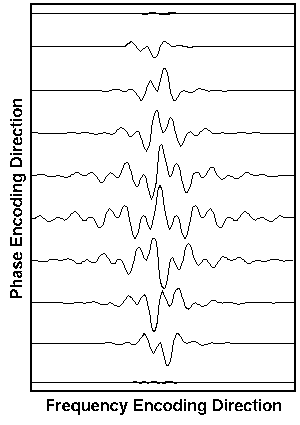
\includegraphics[width=4.5cm]{kSpace}
  }
  \subfigure[Frequency domain information extracted by performing a
    Fourier transform along the x-axis.]{
    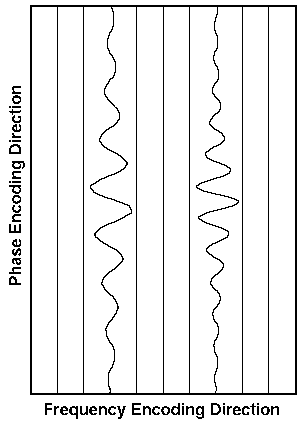
\includegraphics[width=4.5cm]{frequencyDomain}
  }
  \subfigure[Frequency and phase domain information extracted by performing a
    2D Fourier transform along the x- and y-axis.]{
    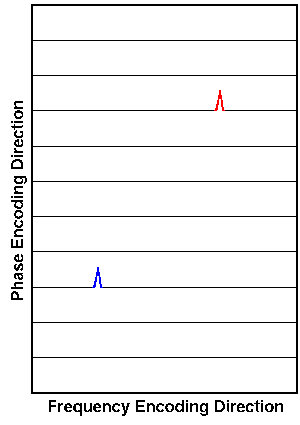
\includegraphics[width=4.5cm]{phaseDomain}
  }
  \caption{The effect from fourier transforming a K-space image.}
  \label{fig:phaseShift}
\end{figure}


% The signal strength is the length of the complex number from the
% fourier transform, not just the real component.


%%% Local Variables:
%%% mode: latex
%%% TeX-master: t
%%% TeX-PDF-mode: t
%%% End:
